%!TEX root = draft.tex
\section{Proving \CRDTLin{}}
\label{sec:proofs}

We describe a proof methodology for showing that CRDT objects are
\crdtlinearizable{}.
This methodology consists in proving an inductive invariant that
entails a simulation based on refinement
mappings~\cite{AbadiL91,DBLP:journals/iandc/LynchV95}, showing that
the evolution of replica states can be simulated by the specification.

\subsection{Proof Methodology}\label{ssec:proof-methodology}

In order to show \crdtlin{} (w.r.t. a specification $\Spec{}$) we start by
instrumenting the object semantics with an auxiliary variable
$\alinord$ recording a linearization of the current history (i.e., the history recorded
in the object's global configurations). 
%This follows a rather standard approach for 
%proving classical linearizability, 
%of~\cite{AbadiL91, VafeiadisHHS06, more citations}.

As explained in \autoref{sec:overview} there are two actions in the
semantics that can modify the state of replicas:
\begin{inparaenum}
\item the execution of a new client request at the origin replica,
  which is shown under the \lstinline|atSource| label -- immediately
  followed by the \lstinline|downStream| at the origin replica
  --, or
\item the execution of the effector of an operation originating in a
  different replica shown under the \lstinline|downStream| label of
  the implementation.
\end{inparaenum}
%
While the execution of an operation at its origin replica represents
the arrival of a new operation, the execution of 
\lstinline|downStream| in a different replica represents the
propagation of effects of preexisting operations.
%
Since the sequence $\alinord$ is a global order over all the
operations of the object in the system, it needs only be updated when
a \emph{new} operation arrives, therefore only during the execution of the code under the
\lstinline|atSource| label\footnote{For readers familiars with proving classical
  linearizability for concurrent objects, this is akin to assuming that
  \lstinline|atSource| is a ``fixed'' linearization point.
  However, differently from the classical case, the operation may not
  be necessarily placed at the end of the current linearization.},
by adding the current operation at some specific position in the
linearization being constructed.
%
%In this paper we only consider CRDTs whose linearizations are
%consistent with the visibility of operations.
%%
%That is, the order of linearization of an execution respects the
%causality of in the execution.\footnote{In fact, we are not aware of
%  \CRDTLinshort{} CRDTs where this is not true.}
%
To guarantee that the linearization is consistent with the visibility
relation, the operation must be inserted in the linearization after
all the operations which are visible at the replica executing
\lstinline|atSource| (we will give later two different strategies for achieving this requirement).
%%
%\gpnote*{Clarify?}
%{
%This guarantees that the linearization $\alinord$ is consistent with
%the visibility relation.
%}
When the object contains query-update operations, the operations are
first rewritten according to a query-update rewriting $\gamma$ as in
\autoref{definition:distributed linearizability} before being placed
in the linearization.
Then, the objective is to prove that $\alinord$ is an
\crdtlinearization{} of the current history (w.r.t. $\Spec{}$), and
this is an invariant for any execution of the object.
%
To prove this invariant, we strengthen it with additional requirements
in order to make it inductive.
%
In the case of the objects we investigated, the inductive invariant is
defined as the conjunction of two properties:
\begin{itemize}
%\setlength{\itemsep}{0.5pt}
\item[-] $\mathsf{ReplicaStates}$: requiring that for each replica
  $\arep$ with local configuration $(\alabelset,\astate)$, the state
  $\sigma$ is obtained by applying the effectors of the operations
  in $\alabelset$ (that have been delivered to $\arep$) \emph{in the order
  defined by $\alinord$} (that is, for any two effectors $\effector_1$ and $\effector_2$ produced by two operations $\alabel_1$ and $\alabel_2$,  
  $\effector_1$ is applied  before $\effector_2$ if $\alabel_1$ is linearized before $\alabel_2$), and
\item[-] $\mathsf{\CRDTLinshort{}}$: requiring that the sequence
  $\alinord$ is an \crdtlinearization{} of the current history (w.r.t.
  $\Spec{}$).
% is \crdtlinearizable{} w.r.t \Spec{} and $\mathit{lin}$ is a
% linearization. Here $\alabelset$ is the set of labels in domain of
% $\downstreams$.
\end{itemize}
To prove that this is an inductive invariant we rely on additional
assertions describing the result of applying each effector (we provide
examples in the following subsections), joint with a proof that:
\begin{itemize}
%\setlength{\itemsep}{0.5pt}
\item[-] $\mathsf{Refinement}$: each effector produced by an operation
  $\alabel$, respectively each query $\alabel$, is simulated by the
  execution of $\alabel$ in the specification $\Spec$. 
\end{itemize}
Essentially, this last requirements establishes a strong
correspondence between the implementation of the algorithm and its
specification. Actually, when using query-updates rewritings $\gamma$, $\mathsf{Refinement}$ requires that 
the effector produced by an operation $\alabel$ be simulated by $\secondrep(\gamma(\alabel))$ 
(the update label in the image of $\alabel$ w.r.t. $\gamma$) in the specification. 

The proof of $\mathsf{Refinement}$ relies on a \emph{refinement
  mapping}~\cite{AbadiL91,DBLP:journals/iandc/LynchV95} between replica states and states of the
specification, denoted by $\refmap$. Intuitively, $\refmap$ being a refinement mapping means that any
effector or query applied on a replica state $\sigma$ can be mimicked by the corresponding operation in the specification
starting from $\refmap(\sigma)$ and leading to a specification state which is related by $\refmap$ to the resulting
replica state.
More precisely, it is required that for 
any two replica states $\sigma$ and $\sigma'$,
\begin{enumerate}
        \item if $\sigma'$ is obtained from $\sigma$ by applying an
          effector $\delta$ produced by an operation $\alabel$, then
          \mbox{$\refmap(\sigma)\specarrow{\alabel}\refmap(\sigma')$},
          where $\specarrow{\alabel}$ is the transition function of
          $\Spec$, or \mbox{$\refmap(\sigma)\specarrow{\secondrep(\gamma(\alabel))}\refmap(\sigma')$} 
          when a query-update rewriting $\gamma$ is used,
          and
        \item if a query $\alabel$ is applied on a state $\sigma$ or
          it is introduced by a rewriting of a query-update that
          executes \lstinline|atSource| on a state $\sigma$, then
          $\refmap(\sigma)\specarrow{\alabel}\refmap(\sigma)$.
\end{enumerate}
% \gpnote*{Explain or remove}{
% Actually, for the CRDT objects presented in \autoref{subsec:time order of execution as linearization}, we consider a stronger version of $\mathsf{Refinement}$ which requires that the state $\sigma$ and the downstream $\delta$ satisfy some particular condition (in the context of the first proof goal).
% }

%\gpnote[nomargin, inline]{Forward reference to exec-order, and
%  ts-order.}

\begin{figure}[t]
%\centering
{\footnotesize
\begin{tabular}{|l|c|r|}
\hline
{\bf CRDT} & {\bf Interface} & {\bf Linearization strategy}\\
\hhline{|===|}
Counter~\cite{ShapiroPBZ11}&$\alabelshort[{\tt inc}]{}$, $\alabelshort[{\tt dec}]{}$ & execution-order \\
\hline
PN-Counter~\cite{ShapiroPBZ11}&$\alabelshort[{\tt inc}]{}$, $\alabelshort[{\tt dec}]{}$ & execution-order \\
\hline
LWW-Register~\cite{DBLP:journals/rfc/rfc677}&$\alabelshort[{\tt write}]{value}$, $\alabellong[{\tt read}]{}{value}{}$ & timestamp-order\\
\hline
Multi-Value Register~\cite{DBLP:conf/sosp/DeCandiaHJKLPSVV07}&$\alabelshort[{\tt write}]{value}$, $\alabellong[{\tt read}]{}{set}{}$ & execution-order\\
\hline
2P-Set~\cite{ShapiroPBZ11}&$\alabelshort[{\tt add}]{value}$, $\alabelshort[{\tt remove}]{value}$, $\alabellong[{\tt read}]{}{set}{}$ & execution-order\\
\hline
LWW-Set~\cite{ShapiroPBZ11}&$\alabelshort[{\tt add}]{value}$, $\alabelshort[{\tt remove}]{value}$, $\alabellong[{\tt read}]{}{set}{}$ & timestamp-order\\
\hline
%PN-set~\cite{ShapiroPBZ11}&not \crdtlinearizable{}&$add$, $remove$, $read$\\
%\hline
OR-Set~\cite{ShapiroPBZ11}&$\alabelshort[{\tt add}]{value}$, $\alabelshort[{\tt remove}]{value}$, $\alabellong[{\tt read}]{}{set}{}$ & execution-order\\
\hline
RGA~\cite{RohJKL11}&$\alabelshort[{\tt addAfter}]{value,value}$, & timestamp-order
                \\ & $\alabelshort[{\tt remove}]{value}$, $\alabellong[{\tt read}]{}{list}{}$ & \\
\hline
Wooki~\cite{DBLP:conf/wise/WeissUM07}&$\alabelshort[{\tt addBetween}]{value,value,value}$, & execution-order
                \\ & $\alabelshort[{\tt remove}]{value}$, $\alabellong[{\tt read}]{}{list}{}$ & \\
\hline
TreeDoc~\cite{DBLP:conf/icdcs/PreguicaMSL09}&$\alabelshort[{\tt addBetween}]{value,value,value}$, & execution-order
                \\ & $\alabelshort[{\tt remove}]{value}$, $\alabellong[{\tt read}]{}{list}{}$ & \\
\hline
\end{tabular}
}
\caption{CRDTs proved RA-linearizable and the linearization strategy used in each case.}
\label{fig:crdt-implementaton of this paper, their correctness, and their interface}
\end{figure}

We have applied this methodology to a range of CRDTs listed in \autoref{fig:crdt-implementaton of this paper, their correctness, and their interface},
including different implementations of counters, registers, sets, and lists. With each CRDT we give its interface which should be self-explanatory
({\tt addBetween} adds a value in between two other values).
We have identified two general classes of
CRDT implementations which differ in the way in which the
linearization $\alinord$ is extended when executing operations at
the origin replica.
For the first class of objects, which includes the OR-Set in
Listing~\ref{lst:or-set}, the linearization $\alinord$ is defined by
the order in which the operations are executed at their origin replica (that is
when \lstinline|atSource| is executed).
In this case a new operation is immediately appended
to the current linearization $\alinord$ (\S~\ref{subsec:time order of execution
  as linearization}).
We say that such objects admit \emph{execution-order linearizations}.
The second class of objects, including the RGA in
Listing~\ref{lst:rga}, supports RA-linearizability proofs in which the
linearization is built based on timestamps, e.g., $\alinord$ is
consistent with the order between the timestamps generated by
operations (\S~\ref{subsec:time-stamp order as linearizabtion}).
We say that such objects admit \emph{timestamp-order linearizations}.
The last column in \autoref{fig:crdt-implementaton of this paper, their correctness, and their interface}
shows the type of linearizations admitted by each of the CRDTs we considered. 
In order to focus on the RA-linearizability proofs we delay the formal definition 
of an object admitting execution-order or timestamp-order linearizations until \autoref{sec:compositionality}.
We will now illustrate these proof strategies using OR-Set and RGA as examples,
%
%We will in each case leave a semi-formal argument for their
%linearizability, 
and explain the commonalities of all other CRDTs in
the same class.
%%
%The formal proofs are relegated to~\autoref{sec:appendix proofs of
%  crdt implementations}.

%
%For some CRDT implementations, when proving its correctness, we can use the total-order of executions as linearization. For such CRDT implementations, our proof approach is as follows:
%
%
%Given a object $\aobj$ and a specification \Spec{}, we construct a predicate $P(\mathit{config},\mathit{lin})$ where $\mathit{config} = (\gstates, \avisord, \downstreams)$ is a configuration of $\llbracket \aobj \rrbracket_{\mathit{op}}$, and $\mathit{lin}$ is a sequence used as linearization. We require $P(\mathit{config},\mathit{lin})$ to be a conjunction of the following statements:
%
%\begin{itemize}
%\setlength{\itemsep}{0.5pt}
%\item[-] Condition $C_1$ (linearizability): The history $(\alabelset, \avisord)$ is \crdtlinearizable{} w.r.t \Spec{} and $\mathit{lin}$ is a linearization. Here $\alabelset$ is the set of labels in domain of $\downstreams$.
%
%\item[-] Condition $C_2$ (downstream): A statement about downstream for each operation label in $\mathit{config}$.
%
%\item[-] Condition $C_3$ (sequential explanation): For each replica $\arep$, we have that $\gstates(\arep).\astate = \mathit{apply}(\mathit{lin},\gstates(\arep).\alabelset)$.
%\end{itemize}
%
%Here the function $\mathit{apply}(\mathit{lin},S)$ returns a local state obtained by applying downstream of operations in $S$ according to total order of $\mathit{lin}$.

\subsection{Execution-Order Linearizations}
\label{subsec:time order of execution as linearization}

%Then, we need to prove that $P$ is a simulation relation. Moreover, we prove that we can always obtain a new linearization by putting a new operation after the tail of a old linearization. We call such relation a execution-order simulation relation.
%
%\begin{itemize}
%\setlength{\itemsep}{0.5pt}
%\item[-] $P(\mathit{config}_0,\epsilon)$ holds, where $\mathit{config}_0$ is the initial configuration.
%
%\item[-] If $P(\mathit{config},\mathit{lin})$ holds and $\mathit{config} {\xrightarrow{\alabel}} \mathit{config}'$, then $P(\mathit{config}', \mathit{lin} \cdot \alabel)$ holds.
%
%\item[-] If $P(\mathit{config},\mathit{lin})$ holds and $\mathit{config} {\xrightarrow{}} \mathit{config}'$, then $P(\mathit{config}',\mathit{lin})$ holds.
%\end{itemize}
%
%It is easy to see that, execution-order simulation relation implies a \crdtlinearizable{} relation proof with the execution as linearization.

In this section, we describe a first instantiation of the methodology described above using as example the OR-Set in Listing~\ref{lst:or-set}. The proof that this CRDT satisfies \crdtlin{} w.r.t. the specification defined in Example~\ref{definition:sequential specification of or-set} relies on several annotations which are given on the lines starting with {\tt //@} in Listing~\ref{lst:or-set} and that we describe hereafter.

%a two-vocabulary formula, the primed, resp., unprimed, variables denoting values after, resp., before, the execution of the procedure.

The annotations included under the \lstinline|atSource| labels describe the construction of the linearization,
%We describe updates of the linearization using \lstinline|let| constructs that append a set of labels.
which is extended by appending operations, after possibly rewriting
them through the query-update rewriting $\gamma$ show in the example of~\ref{fig:or-set-lk-rem}. %, when they execute the \lstinline|atSource| procedure.
The annotations under \lstinline|downStream| specify the behavior of the effectors, e.g., characterizing the result of applying them based on the set of operations visible to the replica where they were generated
% at the moment of applying the corresponding generator 
%this operation has originated 
(at the time when the corresponding generator has been executed). These annotations are written as two-vocabulary formulas, the primed, resp. unprimed, variables denoting values of variables after, resp. before, the execution of the effector. Concretely, the characterization of the effectors corresponding to an {\tt add} operation is self-explanatory (just a logical interpretation of the code under the specific \lstinline|downStream| label) while the characterization of {\tt remove} effectors is more involved. The latter is expressing the fact that 
a {\tt remove} effector removes the set of element-id pairs added by {\tt add} operations visible at the replica $\arep$ where the {\tt remove} originated, and which were not ``canceled'' by other {\tt remove}s visible at $\arep$ ({\tt remove}s that saw those {\tt add} operations).\footnote{This characterization of the set of element-id pairs removed by a {\tt remove} effector is written on the first annotation line under \lstinline|downStream(R)|.}

In the following, we show that the $\mathsf{ReplicaStates}$ property described above is an inductive invariant for OR-Set. Since every operation is appended to the linearization when it executes \lstinline|atSource| it clearly follows, in the linearization order, all operations visible to it. Then, by the causal delivery assumption, the order in which effectors are applied at a given replica is also consistent with the visibility order. 
Therefore, showing that $\mathsf{ReplicaStates}$ is an inductive invariant only requires dealing with the situation where two effectors corresponding to two \emph{concurrent} operations $\alabel_1$ and $\alabel_2$ (i.e., $(\alabel_1,\alabel_2)$ and $(\alabel_2,\alabel_1)$ are not included in the visibility) are applied at some replica in an order that doesn't coincide with the linearization order between $\alabel_1$ and $\alabel_2$. 
%have to be linearized in an order which does not coincide with the order in which their downstreams might have been applied in one or more of the replicas. 
It is important to recall at this point that concurrent operations can be applied in different orders in different replicas. 
% The main difficulty in showing that $\mathsf{ReplicaStates}$ is an inductive invariant is when two downstreams correspond to two ``concurrent'' operations (not related by visibility) and their linearization order is different from the order in which they are applied at a given replica.
% \gpnote*{Refine this text.}
Importantly, a fundamental property of CRDTs~\cite{ShapiroPBZ11} is that the effectors of concurrent operations should \emph{commute}. In other words, applying them in any order leads to the same state.
The fact that concurrent effectors commute is an easy consequence of the annotations under \lstinline|downStream|: two {\tt add} or two {\tt remove} effectors commute obviously because they both add or both remove element-id pairs, while an {\tt add} and a {\tt remove} effector commute when they are concurrent because in this case, the element-id pairs removed by the {\tt remove} effector are different from the pair added by the {\tt add} effector (since the {\tt add} is not visible to {\tt remove}).

The proof of $\mathsf{Refinement}$ is quite straightforward. We consider a refinement mapping $\refmap$ defined as the identity function. For instance, the effector produced by $\alabelshort[{\tt add}]{a,k}$~\footnote{As we mentioned in \autoref{ssec:proof-methodology}, whenever an operation label $\alabel$ is rewritten to another label $\alabel'$, e.g. $\alabelshort[{\tt add}]{a}$ is rewritten to $\alabelshort[{\tt add}]{a,k}$, then the effector produced by the original operation $\alabel$ must be simulated by the operation $\alabel'$ in the specification. Similarly, for query-updates $\alabel$ rewritten to $(\alabel_1,\alabel_2)$, the effector produced by $\alabel$ must be simulated by the operation $\alabel_2$ in the specification.} and the $\alabelshort[{\tt add}]{a,k}$ operation of the specification $\specOrSet$ has exactly the same effect. The same holds for the effector produced by $\alabelshort[{\tt remove}]{a,R}$. Concerning query operations, there are two cases. First, whenever the query-update $\alabelshort[{\tt remove}]{a}$ executes \lstinline|atSource| on a state $\sigma$, the query $\alabellong[{\tt readIds}]{a}{R}{}$ introduced by the query-update rewriting should be enabled in the specification state $\refmap(\sigma)=\sigma$. This clearly holds because the output ${\tt R}$ of ${\tt readIds(a)}$ in the specification is computed exactly as the variable ${\tt R}$ in \lstinline|atSource|.
% the computation of $R$ in \lstinline|atSource| and as the output of $\alabelshort[{\tt readIds}]{a}$ in the specification state $\sigma$ are exactly the same, and (2) 
Second, applying the query $\alabellongind[{\tt read}]{}{A}{}$ on the replica state $\sigma$ should result in the same return value ${\tt A}$ as applying the same query in the context of the specification on the state $\refmap(\sigma)=\sigma$, which again holds trivially.

Finally, we describe the proof of the fact that $\mathsf{\CRDTLinshort{}}$ is an inductive invariant. As already mentioned, appending operations to the linearization when they execute \lstinline|atSource| clearly implies that $\alinord$ is consistent with visibility. Next, the projection of $\alinord$ on the updates is obviously admitted by the specification (the updates are always enabled from the point of view of the specification).
%The only thing to show is that the element-id pairs removed by a {\tt remove} have been added by {\tt adds} which precede it in the linearization, and not already removed by other {\tt remove}s that precede it. This is a direct consequence of the fact that the linearization order is consistent with the visibility relation, and the invariant $\mathsf{ReplicaStates}$, which implies that every element-id pair in a the state of a replica $\arep$ has been added by an {\tt add} visible to $\arep$ and not removed by other {\tt remove}s visible to $\arep$. Then,
Then, we have to argue that queries can be explained by applying the updates visible to them in linearization order (the item~(\ref{it:query}) in  Definition~\ref{definition:ralinearizability1}).
More precisely, we have to show that for each query $\alabel_{\mathsf{qr}}\in\{\alabellongind[{\tt readIds}]{a}{R}{},\alabellongind[{\tt read}]{}{A}{}\}$, the sequence $\alinord'\cdot \alabel_{\mathsf{qr}}$ where $\alinord'$ is the projection of $\alinord$ on the set of updates
visible to $\alabel_{\mathsf{qr}}$ is admitted by the specification. First, by $\mathsf{ReplicaStates}$, the state $\sigma$ of the replica where $\alabel_{\mathsf{qr}}$ is applied is obtained by applying the effectors of the operations visible to $\alabel_{\mathsf{qr}}$ in the linearization order. Then, by $\mathsf{Refinement}$, every effector is simulated by the corresponding operation in the context of the specification. This implies that $\refmap(\sigma_0)\specarrow{\alinord'}\refmap(\sigma)$, where $\sigma_0$ is the initial replica state. The query $\alabel_{\mathsf{qr}}$ is also simulated by the same operation in the context of the specification, which implies that $\refmap(\sigma)\specarrow{\alabel_{\mathsf{qr}}}\refmap(\sigma)$. These two facts imply that $\refmap(\sigma_0)\specarrow{\alinord'\cdot \alabel_{\mathsf{qr}}}\refmap(\sigma)$ which means that $\alinord'\cdot \alabel_{\mathsf{qr}}$ is admitted by the specification.

We give hereafter a formal definition of an RA-linearizable object admitting execution-order linearizations. Intuitively, an object $\aobj$ admits execution-order linearizations when the history of every trace (execution) can be linearized in the order in which operations are executed at the origin replica.

\begin{definition}\label{def:exec_order}
  Let $\aobj$ be an object which is \crdtlinearizable{} w.r.t. a specification $\Spec$. We say that $\aobj$ admits \emph{execution-order linearizations} if for every trace $\atrace\in\traces(\aobj)$ with $\hist{\atrace}=(\alabelset,\avisord)$, there exists an \crdtlinearization{} $(\alabelset,\alinord)$ of $\hist{\atrace}$ w.r.t. $\Spec$ such that $\alabel_1$ occurs before $\alabel_2$ in $\alinord$ iff $\src{}{\alabel_1}$ occurs before $\src{}{\alabel_2}$ in $\atrace$, for every two labels $\alabel_1,\alabel_2\in\alabelset$.
\end{definition}

The following theorem shows the set of objects we have proved to be
RA-linearizable and admit execution-order linearizations (also
mentioned in \autoref{fig:crdt-implementaton of this paper, their
  correctness, and their interface}). The specification of the two
variations of counters is given in Example~\ref{definition:sequential
  specification of counter}. The Multi-Value Register deals with
concurrent write operations by taking the union of the values written
by them (therefore, a {\tt read} operation may return a set of
values).
Its specification is in the same vein as the one of the OR-Set (in particular, a write operation is a query-update since it reads and overwrites the values which are present at the origin replica). The specification of the 2P-Set is a standard Set specification (where ${\tt add}$ and ${\tt remove}$ operations act as in a standard sequential set) while the specifications of Wooki and Treedoc are similar to RGA except that elements are added using the operation ${\tt addBetween}$ which inserts an element in between two other elements. The precise definitions of these specifications and the proofs can be found in the supplementary material. We remark that proving $\mathsf{ReplicaStates}$ and $\mathsf{Refinement}$ in the case of Wooki and Treedoc in particular is more involved than in the case of OR-Set. The concrete replica states are more complex, they are lists or trees of values and metadata, which makes the reasoning about concurrent operations and refinement mappings more challenging.
\begin{theorem}\label{th:execution_order_objects}
Counter, PN-Counter, Multi-Value Register, 2P-Set, OR-Set, Wooki, and Treedoc are RA-linearizable and admit execution-order linearizations.
\end{theorem}

\subsection{Timestamp-Order Linearizations}
\label{subsec:time-stamp order as linearizabtion}

\begin{figure}[t]
  \centering
  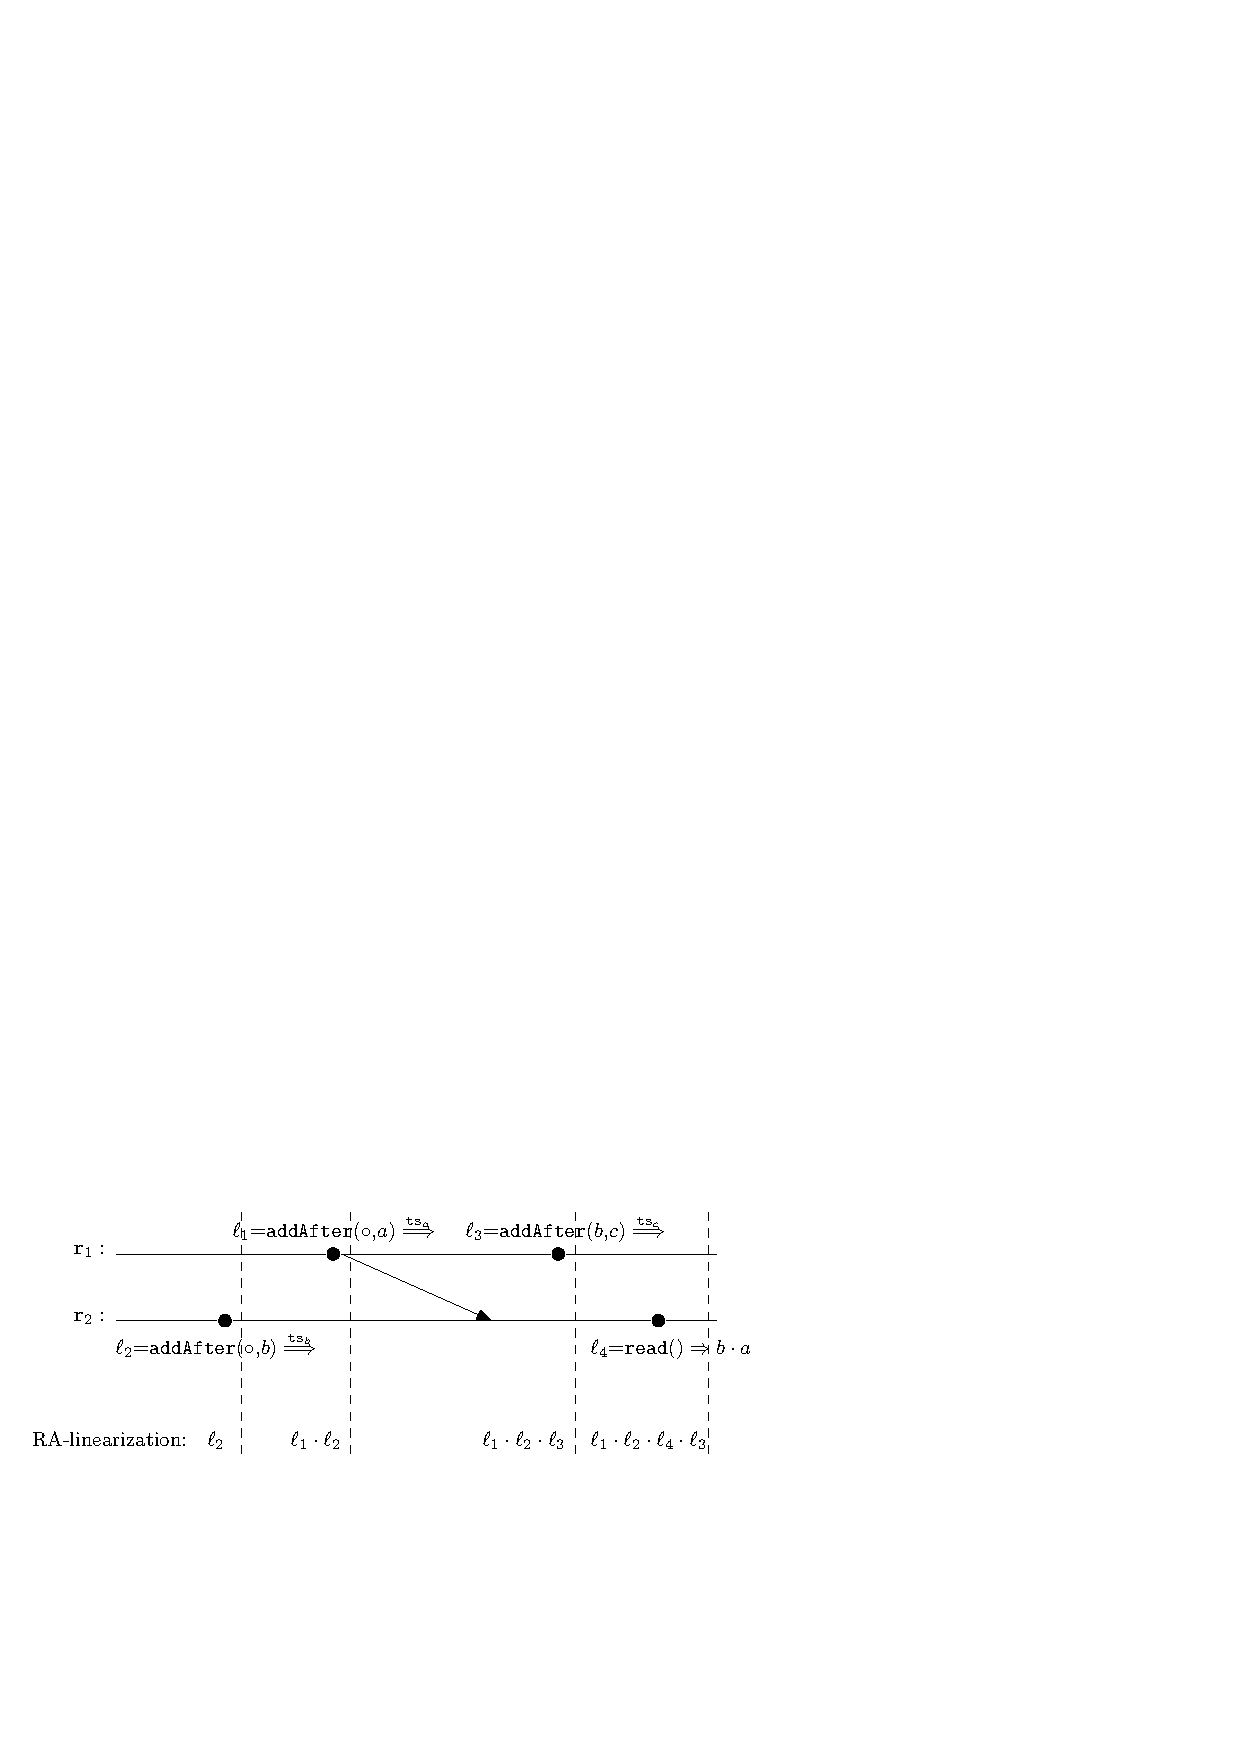
\includegraphics[width=0.7 \textwidth]{figures/RGAHisandLin.pdf}
%\vspace{-10pt}
  \caption{An execution of RGA and the corresponding execution-order and timestamp-order linearizations. We assume that $\ats_a<\ats_b<\ats_c$.}
  \label{fig:a history of RGA and its RA-linearization}
\end{figure}

CRDT objects such as RGA in Listing~\ref{lst:rga}, that use timestamps for conflict resolution, may not admit execution-order linearizations. 
For instance, \autoref{fig:a history of RGA and its RA-linearization} shows an execution of RGA where two replicas $\arep_1$ and $\arep_2$ execute two ${\tt addAfter}$ invocations, and an ${\tt addAfter}$ invocation followed by a ${\tt read}$ invocation, respectively. An execution-order linearization which by definition, is consistent with the order in which the operations are applied at the origin replica, will order $\alabelshort[{\tt addAfter}]{\circ,b}$ before $\alabelshort[{\tt addAfter}]{\circ,a}$. The result of applying these two operations in this order in the specification $\specRGA$ (defined in Example~\ref{definition:sequential specification of rga}) is the list $a\cdot b$. However, as explained in \autoref{sec:rga-crdt-impl}, assuming that the timestamp $\ats_a$ associated to the element $a$ is smaller than the timestamp $\ats_b$ associated to $b$, the query ${\tt read}$ that sees these two operations will return the list $b\cdot a$, which is different than the one obtained by applying the same operations in the context of $\specRGA$ in linearization order. This shows that such a linearization is not a valid RA-linearization (w.r.t. $\specRGA$).
To prove that such objects are \crdtlinearizable{}, we consider another instantiation of the proof methodology described in \autoref{ssec:proof-methodology} where the linearization is additionally \emph{consistent with the order of timestamps} generated by the operations.
We describe this instantiation using the RGA as an example (showing that it is RA-linearizable w.r.t. $\specRGA$).

%\gpnote{I think this example is kinda complicated. Maybe add picture?}
The construction of the linearization ensures that the operations that generate a timestamp, i.e., the invocations of ${\tt addAfter}$, are ordered in the linearization according to their timestamps. For instance, if we consider the execution in \autoref{fig:a history of RGA and its RA-linearization}, $\alabelshort[{\tt addAfter}]{\circ,a}$ will be ordered before $\alabelshort[{\tt addAfter}]{\circ,b}$ because $\ats_a$ is smaller than $\ats_b$ (even though they are executed in a different order at their origin replica). 
%More precisely, for any two operations $\alabelshort[{\tt addAfter}]{a,b}$ and $\alabelshort[{\tt addAfter}]{c,d}$ that generate two timestamps $\ats_{\tt b}$ and $\ats_{\tt d}$, respectively, the linearization should order $\alabelshort[{\tt addAfter}]{a,b}$ before $\alabelshort[{\tt addAfter}]{c,d}$ if $\ats_{\tt b}<\ats_{\tt d}$ and $\alabelshort[{\tt addAfter}]{c,d}$ before $\alabelshort[{\tt addAfter}]{a,b}$ if $\ats_{\tt d}<\ats_{\tt b}$. 
%
Moreover, to extend the notion of timestamp ordering to operations $\alabel$ that don't generate timestamps, i.e., invocations of ${\tt remove}$ and ${\tt read}$, we consider a ``virtual'' timestamp which is defined as the \emph{maximal} timestamp of any operation visible to $\alabel$ (or $\bot$ if no operation is visible to $\alabel$), and then require that the linearization is consistent with the order between both ``real''~\footnote{That is, timestamps generated by the operation itself.} and ''virtual'' timestamps. For instance, the {\tt read} operation in \autoref{fig:a history of RGA and its RA-linearization} sees $\alabelshort[{\tt addAfter}]{\circ,a}$ and $\alabelshort[{\tt addAfter}]{\circ,b}$, therefore, its ``virtual'' timestamp is $\ats_b$. Then, a valid RA-linearization will order the {\tt read} operation before the other $\alabelshort[{\tt addAfter}]{b,c}$ operation, since the timestamp $\ats_c$ of the latter is bigger than the ``virtual'' timestamp $\ats_b$ of the {\tt read}. The operations that have the same timestamp~\footnote{Among operations that have the same timestamp $\ats$, there is exactly one operation generating $\ats$, the rest of the operations having $\ats$ as a ``virtual'' timestamp (i.e., they don't generate timestamps themselves and the maximal timestamp they see is $\ats$).} are ordered as they execute at the origin replica. For instance, the {\tt read} operation with timestamp $\ats_b$ is ordered after $\alabelshort[{\tt addAfter}]{\circ,b}$ that has the same timestamp $\ats_b$ since it executes later at the origin replica.


The annotations defining the linearization are included under the \lstinline|atSource| labels of~\autoref{lst:rga}. The function {\tt insert}($\alinord$,$\alabel$,$\ats$) inserts the label $\alabel$ in the linearization $\alinord$ just after the last operation $\alabel'$ in $\alinord$ which has a timestamp (real or virtual) smaller than or equal to $\ats$. The annotations characterizing the effectors are quite straightforward in this case, since they are straightforward logical interpretations of the program statements.

The proof of $\mathsf{ReplicaStates}$ is quite similar to the case of OR-Set. Since the order between the timestamps generated by ${\tt addAfter}$ operations is consistent with the visibility relation (see \autoref{ssec:semantics}), it easily follows that the linearization order $\alinord$ is also consistent with the visibility relation. Then, as in the case of OR-Set, it remains to prove that any two effectors that correspond to two ``concurrent'' operations (not related by visibility) commute. This easily follows from the fact that the effectors apply set union which is obviously commutative. Also, note that by the causal delivery assumption and the preconditions of ${\tt addAfter}$ and ${\tt remove}$, it cannot happen that an $\alabelshort[{\tt addAfter}]{a,b}$ operation adding ${\tt b}$ after ${\tt a}$ is concurrent with an operation that adds ${\tt a}$ to the list, i.e., $\alabelshort[{\tt addAfter}]{c,a}$, for some ${\tt c}$, or that an $\alabelshort[{\tt addAfter}]{a,b}$ operation adding ${\tt b}$ is concurrent with an operation $\alabelshort[{\tt remove}]{b}$ that removes ${\tt b}$. This ensures that reordering concurrent effectors doesn't lead to ``invalid'' replica states where for instance, the timestamp tree ${\tt N}$ contains nodes which are not reachable from the root (which would happen if $\alabelshort[{\tt addAfter}]{a,b}$ is delivered before the operation $\alabelshort[{\tt addAfter}]{c,a}$ adding ${\tt a}$), or where the tombstone set ${\tt Tomb}$ contains elements which are not in the tree (which would happen if $\alabelshort[{\tt remove}]{b}$ is delivered before $\alabelshort[{\tt addAfter}]{a,b}$).

%{\color {red} CW: Each abstract state is in the form $\abstate = (a_1,flag_1) \cdot \ldots \cdot (a_n,flag_n)$.} 
Concerning the proof of $\mathsf{Refinement}$, we consider a refinement mapping $\refmap$ which relates a replica state ${\tt (N,Tomb)}$ with a specification state $(l,T)$ where the sequence of elements $l$ is given by the function ${\tt traverse}$ used in ${\tt read}$ operations by ignoring tombstones, i.e., $l={\tt traverse(N, \emptyset)}$, and $T={\tt Tomb}$. The fact that effectors of ${\tt remove}$ operations, and ${\tt read}$ queries are simulated by the corresponding operations of the specification is straightforward. Concerning effectors of $\alabellongind[{\tt addAfter}]{a,b}{}{\ats_b}{}$ operations, we show that they are simulated by the corresponding specification operation $\alabelshort[{\tt addAfter}]{a,b}$ only when the timestamp $\ats_{\tt b}$ is strictly greater than all the timestamps stored in the replica state where it applies. This is sufficient because, by $\mathsf{ReplicaStates}$, every replica state is obtained by applying effectors according to the linearization of their corresponding operations, and the linearization order is consistent with the timestamp order. Thus, let $({\tt N},{\tt Tomb})$ be a replica state such that $\ats_{\tt a} < \ats_{\tt b}$ for every $\ats_{\tt a}$ with $({\tt c},\ats_{\tt a},{\tt a})\in {\tt N}$ for some ${\tt c}$. The result of applying the effector $\effector$ corresponding to $\alabellongind[{\tt addAfter}]{a,b}{}{\ats_b}{}$ is to add ${\tt b}$ as a child of ${\tt a}$. Then, applying ${\tt traverse}$ on the new state will result in a sequence where ${\tt b}$ is placed just after ${\tt a}$ because it has the biggest timestamp among the children of ${\tt a}$ (and all the nodes in the tree ${\tt N}$). This corresponds exactly to the sequence obtained by applying the operation $\alabelshort[{\tt addAfter}]{a,b}$ in the context of the specification.

To prove that $\mathsf{\CRDTLinshort{}}$ is an inductive invariant, we use almost the same arguments as in the case of OR-Set. The two notable differences are that in this case, the specification doesn't admit any sequence of updates and also, that effectors of ${\tt addAfter}$ operations are simulated by the corresponding specification operations only under a certain condition related to timestamps. Concerning the first point, the specification requires that any $\alabelshort[{\tt addAfter}]{a,b}$ or $\alabelshort[{\tt remove}]{a}$ operation is preceded by an operation adding ${\tt a}$. However, since $\alinord$ is consistent with the visibility relation, and the preconditions of the RGA $\alabelshort[{\tt addAfter}]{a,b}$ and $\alabelshort[{\tt remove}]{a}$ operations ensure that an operation $\alabelshort[{\tt addAfter}]{c,a}$, for some ${\tt c}$, is visible when applying them at the origin replica, it follows that the projection of $\alinord$ on updates is admitted by the specification. Second, we have to show that the side-condition added to the simulation of ${\tt addAfter}$ effectors still guarantees that any sequence $\mathsf{effSeq}$ of effector applications consistent with the linearization order (considering only such sequences is possible because of the $\mathsf{ReplicaStates}$ invariant) can be simulated by the specification. This follows from the fact that the linearization order is consistent with the timestamps generated by operations, which implies that any ${\tt addAfter}$ effector adding an element ${\tt b}$ with timestamp $\ats_{\tt b}$ is ordered in $\mathsf{effSeq}$ after all ${\tt addAfter}$ effectors adding elements with timestamps smaller than $\ats_{\tt b}$.

Next, we present a formal definition of timestamp-order linearizations. For a history $\ahist=(\alabelset,\avisord)$, we define the timestamp $\tsof_\ahist(\alabel)$ of a label $\alabel$ in the context of the history $h$ to be $\tsof_\ahist(\alabel)=\tsof(\alabel)$ if $\tsof(\alabel)\neq\bot$ and $\tsof_\ahist(\alabel)=\mathsf{max}\, \{\tsof(\alabel'):(\alabel',\alabel)\in \avisord \}$, otherwise.

\begin{definition}
An object $\aobj$ which is \crdtlinearizable{} w.r.t. a specification $\Spec$ admits \emph{timestamp-order linearizations} if for every trace $\atrace\in\traces(\aobj)$ with $\hist{\atrace}=(\alabelset,\avisord)$, there exists an \crdtlinearization{} $(\alabelset,\alinord)$ of $\hist{\atrace}$ w.r.t. $\Spec$ such that $\alabel_1$ occurs before $\alabel_2$ in $\alinord$ iff $\tsof_\ahist(\alabel_1) < \tsof_\ahist(\alabel_2)$ or $\src{}{\alabel_1}$ occurs before $\src{}{\alabel_2}$ in $\atrace$, for every two labels $\alabel_1,\alabel_2\in\alabelset$.
\end{definition}

The following theorem shows the set of objects we have proved to be RA-linearizable and admit timestamp-order linearizations (also mentioned in \autoref{fig:crdt-implementaton of this paper, their correctness, and their interface}). The specification of the LWW-register (short for Last Writer Wins Register) is standard, i.e., a read operation returns the last written value, while the specification of the LWW-Set is similar, the object storing a set of values instead of a single value like in the context of the LWW-register. The precise definitions of these specifications and the proofs can be found in the supplementary material.

\begin{theorem}\label{th:ts_order_objects}
LWW-Register, LWW-Set, and RGA are RA-linearizable and admit timestamp-order linearizations.
\end{theorem}

TODO SAY THAT RGA WITH ADDAT IS NOT RA-LINEARIZABLE

%%% Local Variables:
%%% mode: latex
%%% TeX-master: "draft"
%%% End:
